\documentclass[a4paper,12pt]{book}
\usepackage[utf8]{inputenc}
\usepackage{graphicx}
\usepackage[spanish]{babel}
\usepackage{color}
\usepackage[table]{xcolor}
\usepackage{hyperref}
\usepackage[numbered]{bookmark}
\usepackage{fancyhdr}
\usepackage{fancybox}
\usepackage{longtable}
\usepackage{amsmath}
\usepackage{titlesec}
\definecolor{gray97}{gray}{.97}
\definecolor{gray75}{gray}{.75}
\definecolor{gray45}{gray}{.45}

% Set the Paper Size and margins
\RequirePackage{geometry}
\geometry{margin=0.9in,bottom=1.7in}

\hypersetup{colorlinks=true,
	linkcolor=black,
	citecolor=blue,
	filecolor=black,
	urlcolor=blue,
	pdfauthor=  Luis Andrés Valido Fajardo
}


\newcommand{\universidad}{\large{Universidad de Matanzas }}
\newcommand{\facultad}{\large{Departamento de Recursos para el Aprendizaje}}

\newcommand{\espacios}{\vspace{0.5in}}

\newcommand{\espaciosH}{\hspace{0.5in}}

\newcommand{\titleguide}[1]{\gdef\@titleguide{#1}}

\newcommand{\uchapter}[1]{\chapter*{#1}
	\addcontentsline{toc}{section}{\protect\numberline{}#1}}

\newcommand{\usection}[1]{\section*{#1}
	\addcontentsline{toc}{section}{\protect\numberline{}#1}}

\newcommand{\usubsection}[1]{\subsection*{#1}
	\addcontentsline{toc}{subsection}{\protect\numberline{}#1}}

\newcommand{\usubsubsection}[1]{\subsubsection*{#1}
	\addcontentsline{toc}{subsubsection}{\protect\numberline{}#1}}


\newcommand{\entidad}
{
 	\begin{tabular}{c}
 		
 		\universidad \\
 		\facultad \\ 
 		\espacios \\
 		
 	\end{tabular}
}

\newcommand{\logoACM}{
\includegraphics[scale=0.7]{img/icpc.png}}
\newcommand{\banner}
{
 \espacios

\begin{tabular}{ccc}

\logoUniversidad  &  \entidad  &  \logoFacultad  \\

\end{tabular}


 \espacios
 }


% Escribir el titulo de la tesis que va a exponer.
\newcommand{\tituloTesis}{Manual de preparación para estudiantes preuniversitarios concursantes del ICPC y IOI en la provincia de Matanzas }

% Cambiar el tipo de trabajo si es necesario.
\newcommand{\nombreTipoTesis}{}

% Cambiar los nombres de los autores.
\newcommand{\autorTemaUNO}{Ernesto Ojea Torres}
\newcommand{\autorTemaTRES}{Luis Alejandro Arteaga Morales}
\newcommand{\autorTemaDOS}{Luis Andrés Valido Fajardo}
\newcommand{\autorTemaCUATRO}{Frank Hernández González}

\newcommand{\analistaUNO}{Luis Andrés Valido Fajardo}
\newcommand{\analistaDOS}{Ernesto David Escariz Ramos}
\newcommand{\analistaTRES}{Luis Alejandro Arteaga Morales}
\newcommand{\analistaCUATRO}{Roniel Navarro Villa}
\newcommand{\analistaCINCO}{Leonardo Fundora Luis}
\newcommand{\analistaSEIS}{Leyán Robaina Mesa}

\newcommand{\correctoreUNO}{Arian Amadeo Castellanos Rodriguez}
\newcommand{\correctoreDOS}{Zaniel García Orihuela}


% Cambiar el cargo del tutor y co-tutor
\newcommand{\cargoTutor}{Cargo del tutor}
\newcommand{\cargoCoTutor}{Cargo del co-tutor}

% Cambiar la fecha de confección de la tesis. Por defecto es el día de hoy
\newcommand{\fecha}{\large{\today}}

\newcommand{\titulo}{ \centering	\large{\bf \tituloTesis}\espacios}

\newcommand{\tipoTesis}{\large{\nombreTipoTesis}\espacios}

\newcommand{\autores}
{
    
    \begin{tabular}{ll}
    \large{\bf Autor de temas:}  &  \large{\autorTemaDOS} \\
                          
   
    
     
    \end{tabular}

 \vspace{0.5in}

	% \begin{tabular}{ll}
	
		
	%	\large{\bf Correciones:}    & \large{\correctoreUNO}    \\
	%	                            & \large{\correctoreDOS} \\
		
		
	%\end{tabular}

    \vspace{0.5in}
    
     \begin{tabular}{ll}
    
    	
    	\large{\bf Análisis de ejercicios:}    & \large{\analistaUNO} \\    
    \end{tabular}
}

\newcommand{\ciudadFecha}{\large{\bf Matanzas, \fecha}}

\newcommand{\fillDia}{\makebox[0.3in]{\hrulefill}\space}
\newcommand{\fillMes}{\makebox[1in]{\hrulefill}\space}
\newcommand{\fillAnno}{\makebox[0.5in]{\hrulefill}}

\newcommand{\firma}{\makebox[2in]{\hrulefill}}

\newcommand{\firmaTesis}
{
    \begin{center}
    \begin{tabular}{cp{0.5in}c}
        \firma      &   & \firma        \\
        \firma      &   & \firma        \\
        \cargoTutor &   & \cargoCoTutor \\
        \tutor      &   & \coTutor
    \end{tabular}
    \end{center}
}

\newcommand{\comentario}[2][]
{
	\todo[caption={#2}, size=\small, #1, inline,color={red!100!green!8},bordercolor=red,linecolor=red]
	{
	  \renewcommand{\baselinestretch}{1.2}\selectfont#2\par
	}
}

\usepackage{listings}
\lstset{ frame=Ltb,
framerule=0pt,
aboveskip=0.5cm,
framextopmargin=1pt,
framexbottommargin=1pt,
framexleftmargin=0.4cm,
framesep=0pt,
rulesep=.4pt,
backgroundcolor=\color{white},
rulesepcolor=\color{black},
%
stringstyle=\ttfamily,
showstringspaces = false,
basicstyle=\small\ttfamily,
commentstyle=\color{blue},
keywordstyle=\bfseries,
%
numbers=none,
numbersep=20pt,
numberstyle=\tiny,
numberfirstline = false,
breaklines=true,
}
% minimizar fragmentado de listados
\lstnewenvironment{listing}[1][]
{\lstset{#1}\pagebreak[0]}{\pagebreak[0]}
\lstdefinestyle{consola}
{basicstyle=\scriptsize\bf\ttfamily,
backgroundcolor=\color{white},
}
\lstdefinestyle{C++}
{language=C++,
}



%\titleformat{\chapter}{\huge}{\MakeUppercase{\thechapter}}{0.2 em}{}
\titlespacing{\chapter}{0pt}{0pt}{10pt}
\titleformat{\chapter}{}{}{0em}{\bf\LARGE}

\begin{document}


\begin{titlepage}
    \begin{center}

%   Logo de la universidad
  %  \banner

%   Titulo de la tesis:
    \titulo

%   Tipo de tesis:
    \tipoTesis

	\logoACM

	\vspace{200pt}
%   Autores y tutores de la tesis
    
    
%   Lugar y fecha de confección de la tesis
    \ciudadFecha

    \end{center}
\end{titlepage}

\autores



\tableofcontents

%\pagebreak
\pagestyle{fancy}
\lhead{}
\chead{}
\rhead{\MakeUppercase{\textit{ Prólogo}}}
\chapter*{Prólogo}
\addcontentsline{toc}{chapter}{\large Prólogo} 
El siguiente documento es una versión mejorada de muchos que comenzaron siendo un simple .txt donde tenía la mala costumbre de colocar el nombre del ejercicio, por la temática por la cual lo había resuelto y el jurado donde lo había solucionado. Creo por ahora este ha superado por mucho los anteriores, quizá dentro de algún tiempo lo vea horrendo. Tuve la necesidad de retomarlo por dos cuestiones. La primera, no se imaginan cuanto me pesaba tener que
implementar desde cero ciertos algoritmos sabiendo que los había hecho con anterior para otros ejercicios, así que comencé anotar por temática los ejercicio que iba resolviendo, no es lo mismo tener que hacer la rueda desde cero, a decir creo que para este ejercicio puede coger la rueda de otro y solo tengo pintarla o cambiar el tipo de goma. Lo segundo para ayudar muchachos sobre todo de la  que se iniciaban en este mundillo.

La estructura del documento esta acorde según mi punto de vista a las principales áreas que debe dominar un concursante de programación. Dentro de cada área abordaré aquellas temáticas o puntos que de cierta manera domino aunque sea lo básico y que al menos tenga un ejemplo de problema en algún jurado que lo solucione usando ese conocimiento. No obstante si alguien cree que faltó algo que debe ser incluido y se siente en condiciones de abordarlo sin problema se puede poner en contacto conmigo (luis.valido@umcc.cu, luis.valido1989@gmail.com) e incluyó su aporte a este documento.  

Cada capítulo termina con el análisis de problemas los cuales se enmarca dentro temas tratados en el capítulo. De no existir ninguna especificación se puede asumir que la solución fue hecha en C++ y el veredicto de ese análisis fue aceptado en ese momento. Bueno creo que por ahora no hay nada más que aclarar. Creo que la cantidad de puntos que pierdo por una ortografía no estandarizada es aceptable por la cantidad de puntos que pueden otorgar los conocimientos aquí expuestos (No obstante se aceptan correciones).Importante casi lo olvidaba este documento digamos que es un beta que se va ir llenando a medida de las posibilidades de tiempo de los autores así que puede encontrar temáticas con solamente el nombre, eso significa que ya se pensado abordarlo lo que aún no se ha tenido el tiempo.




\pagestyle{fancy}
\lhead{}
\chead{}
\rhead{\MakeUppercase{\textit{ Un poco de historia}}}
\chapter*{Un poco de historia}
\addcontentsline{toc}{chapter}{\large Un poco de historia}





\begin{minipage}{0.2\textwidth}
	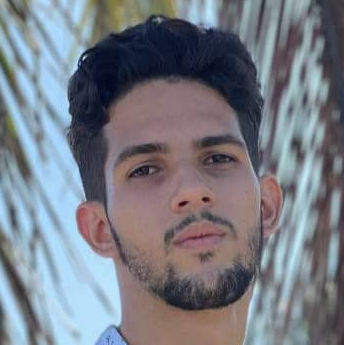
\includegraphics[width=\linewidth]{img/concursantes/alejandro.png} % Replace 'example-image' with the filename of your image
\end{minipage}
\hfill
\begin{minipage}{0.7\textwidth}
	\textbf{Luis Alejandro Arteaga Morales}
	
	\vspace*{0.1in}
	\begin{tabular}{rl}
	
		\textbf{10$^{mo}$} & Bronce en la Copa Regional IPVCE.  \\
		
		\textbf{11$^{no}$} & Medalla de Bronce en el concurso nacional de informática \\
		
		\textbf{12$^{ce}$} & Preselección nacional de informática  \\
		                   & Participó en la Olimpiada Iberoamericana de Informática  \\
		                   & Mención en la Olimpiada Iberoamericana de Informática  \\
		                   & Bronce en el ICPC entre los equipos preuniversitario  \\
		
	\end{tabular}
	
\end{minipage}

\begin{minipage}{0.2\textwidth}
	
\includegraphics[width=\linewidth]{img/icpc.png} % Replace 'example-image' with the filename of your image
\end{minipage}
\hfill
\begin{minipage}{0.7\textwidth}
	\textbf{Marcos Cepero}
	
	\vspace*{0.1in}
	\begin{tabular}{rl}
		
		\textbf{10$^{mo}$} &   \\
		
		\textbf{11$^{no}$} &  \\
		
		\textbf{12$^{ce}$} &   \\
		
		
	\end{tabular}
	
\end{minipage}

\begin{minipage}{0.2\textwidth}
	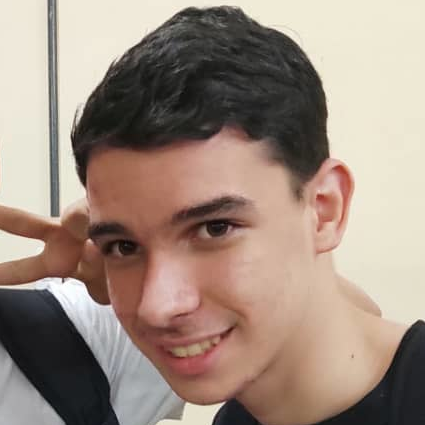
\includegraphics[width=\linewidth]{img/concursantes/leyan.png} % Replace 'example-image' with the filename of your image
\end{minipage}
\hfill
\begin{minipage}{0.7\textwidth}
	\textbf{Leyán Robaina Mesa}
	
	\vspace*{0.1in}
	\begin{tabular}{rl}
		
		\textbf{10$^{mo}$} &   \\
		
		\textbf{11$^{no}$} &  \\
		
		\textbf{12$^{ce}$} &   \\
		
		
	\end{tabular}
\end{minipage}

\begin{minipage}{0.2\textwidth}
	
\includegraphics[width=\linewidth]{img/icpc.png} % Replace 'example-image' with the filename of your image
\end{minipage}
\hfill
\begin{minipage}{0.7\textwidth}
	\textbf{Ahmed Rodríguez Martínez}
	
	\vspace*{0.1in}
	\begin{tabular}{rl}
		
		\textbf{10$^{mo}$} &   \\
		
		\textbf{11$^{no}$} &  \\
		
		\textbf{12$^{ce}$} &   \\
		
		
	\end{tabular}
\end{minipage}

\begin{minipage}{0.2\textwidth}
	
\includegraphics[width=\linewidth]{img/icpc.png} % Replace 'example-image' with the filename of your image
\end{minipage}
\hfill
\begin{minipage}{0.7\textwidth}
	\textbf{José Alejandro Albanés Febles }
	
	\vspace*{0.1in}
	\begin{tabular}{rl}
		
		\textbf{10$^{mo}$} &   \\
		
		\textbf{11$^{no}$} &  \\
		
		\textbf{12$^{ce}$} &   \\
		
		
	\end{tabular}
\end{minipage}


\begin{minipage}{0.2\textwidth}
	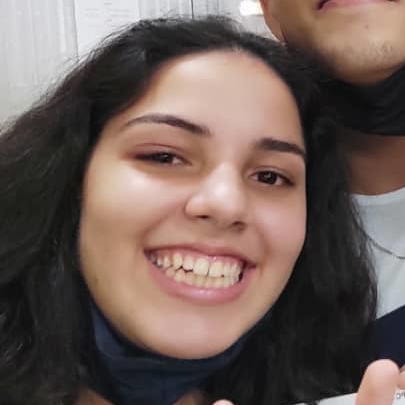
\includegraphics[width=\linewidth]{img/concursantes/alejandra.png} % Replace 'example-image' with the filename of your image
\end{minipage}
\hfill
\begin{minipage}{0.7\textwidth}
	\textbf{Alejandra Tudela Lara}
	
	\vspace*{0.1in}
	\begin{tabular}{rl}
		
		\textbf{10$^{mo}$} &   \\
		
		\textbf{11$^{no}$} &  \\
		
		\textbf{12$^{ce}$} &   \\
		
		
	\end{tabular}
\end{minipage}

\begin{minipage}{0.2\textwidth}
	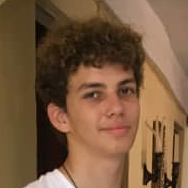
\includegraphics[width=\linewidth]{img/concursantes/daniel.png} % Replace 'example-image' with the filename of your image
\end{minipage}
\hfill
\begin{minipage}{0.7\textwidth}
	\textbf{Daniel Alejandro Estupiñan Reyes}
	
	\vspace*{0.1in}
	\begin{tabular}{rl}
		
		\textbf{10$^{mo}$} &   \\
		
		\textbf{11$^{no}$} &  \\
		
		\textbf{12$^{ce}$} &   \\
		
		
	\end{tabular}
\end{minipage}

\begin{minipage}{0.2\textwidth}
	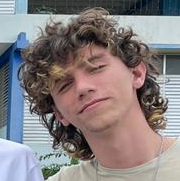
\includegraphics[width=\linewidth]{img/concursantes/adrian.png} % Replace 'example-image' with the filename of your image
\end{minipage}
\hfill
\begin{minipage}{0.7\textwidth}
	\textbf{Adrian Pacheco Rubio}
	
	\vspace*{0.1in}
	\begin{tabular}{rl}
		
		\textbf{10$^{mo}$} &   \\
		
		\textbf{11$^{no}$} &  \\
		
		\textbf{12$^{ce}$} &   \\
		
		
	\end{tabular}
\end{minipage}

\begin{minipage}{0.2\textwidth}
	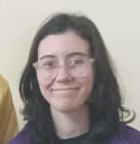
\includegraphics[width=\linewidth]{img/concursantes/karen.png} % Replace 'example-image' with the filename of your image
\end{minipage}
\hfill
\begin{minipage}{0.7\textwidth}
	\textbf{Karen Negrín Mazaría}
	
	\vspace*{0.1in}
	\begin{tabular}{rl}
		
		\textbf{10$^{mo}$} &   \\
		
		\textbf{11$^{no}$} &  \\
		
		\textbf{12$^{ce}$} &   \\
		
		
	\end{tabular}
\end{minipage}



\begin{minipage}{0.2\textwidth}
	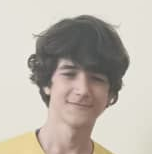
\includegraphics[width=\linewidth]{img/concursantes/reynier.png} % Replace 'example-image' with the filename of your image
\end{minipage}
\hfill
\begin{minipage}{0.7\textwidth}
	\textbf{Reynier García Montes de Oca}
	
	\vspace*{0.1in}
	\begin{tabular}{rl}
		
		\textbf{10$^{mo}$} &   \\
		
		\textbf{11$^{no}$} &  \\
		
		\textbf{12$^{ce}$} &   \\
		
		
	\end{tabular}
\end{minipage}

\begin{minipage}{0.2\textwidth}
	
\includegraphics[width=\linewidth]{img/icpc.png} % Replace 'example-image' with the filename of your image
\end{minipage}
\hfill
\begin{minipage}{0.7\textwidth}
	\textbf{Cristian Ernesto Lugo}
	
	\vspace*{0.1in}
	\begin{tabular}{rl}
		
		\textbf{10$^{mo}$} &   \\
		
		\textbf{11$^{no}$} &  \\
		
		\textbf{12$^{ce}$} &   \\
		
		
	\end{tabular}
\end{minipage}

\begin{minipage}{0.2\textwidth}
	
\includegraphics[width=\linewidth]{img/icpc.png} % Replace 'example-image' with the filename of your image
\end{minipage}
\hfill
\begin{minipage}{0.7\textwidth}
	\textbf{César Raúl Luis González}
	
	\vspace*{0.1in}
	\begin{tabular}{rl}
		
		\textbf{10$^{mo}$} &   \\
		
		\textbf{11$^{no}$} &  \\
		
		\textbf{12$^{ce}$} &   \\
		
		
	\end{tabular}
\end{minipage}

\begin{minipage}{0.2\textwidth}
	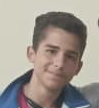
\includegraphics[width=\linewidth]{img/concursantes/oscar.png} % Replace 'example-image' with the filename of your image
\end{minipage}
\hfill
\begin{minipage}{0.7\textwidth}
	\textbf{Oscar Manuel Reyes Mora}
	
	\vspace*{0.1in}
	\begin{tabular}{rl}
		
		\textbf{10$^{mo}$} &   \\
		
		\textbf{11$^{no}$} &  \\
		
		\textbf{12$^{ce}$} &   \\
		
		
	\end{tabular}
\end{minipage}

\begin{minipage}{0.2\textwidth}
	
\includegraphics[width=\linewidth]{img/icpc.png} % Replace 'example-image' with the filename of your image
\end{minipage}
\hfill
\begin{minipage}{0.7\textwidth}
	\textbf{Ronnie Molina Martínez}
	
	\vspace*{0.1in}
	\begin{tabular}{rl}
		
		\textbf{10$^{mo}$} &   \\
		
		\textbf{11$^{no}$} &  \\
		
		\textbf{12$^{ce}$} &   \\
		
		
	\end{tabular}
\end{minipage}

\begin{minipage}{0.2\textwidth}
	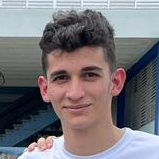
\includegraphics[width=\linewidth]{img/concursantes/zaniel.png} % Replace 'example-image' with the filename of your image
\end{minipage}
\hfill
\begin{minipage}{0.7\textwidth}
	\textbf{Zaniel García Orihuela}
	
	\vspace*{0.1in}
	\begin{tabular}{rl}
		
		\textbf{9$^{no}$} &  \\
		
		\textbf{10$^{mo}$} &   \\
		
		\textbf{11$^{no}$} &  \\
		
		\textbf{12$^{ce}$} &   \\
		
		
	\end{tabular}
\end{minipage}



\lhead{}
\chead{}
\rhead{\MakeUppercase{\textit{ Aritmética Álgebra}}}
\chapter*{\MakeUppercase{\textit{ Aritmética Álgebra}}}
\addcontentsline{toc}{chapter}{\MakeUppercase{\textit{ Aritmética Álgebra}}}

\chapter{Sucesión de Fibonacci}
\section{Introducción}
\input{tex_files/introduccion_fibonacci.tex}
\section{Conocimientos previos}
\input{tex_files/conocimientos_fibonacci.tex}
\section{Desarrollo}
\input{tex_files/desarrollo_fibonacci.tex}
\section{Implementación}
\input{tex_files/code_fibonacci.tex}
\section{Aplicaciones}
\input{tex_files/aplicaciones_fibonacci.tex}
\section{Complejidad}
\input{tex_files/complejidad_fibonacci.tex}
\section{Ejercicios}
\input{tex_files/excercises_fibonacci.tex}


\lhead{}
\chead{}
\rhead{\MakeUppercase{\textit{ Estructura de Datos}}}
\chapter*{\MakeUppercase{\textit{ Estructura de Datos}}}
\addcontentsline{toc}{chapter}{\MakeUppercase{\textit{ Estructura de Datos}}}
\chapter{Árboles y sus propiedades básicas}
\section{Introducción}
\input{tex_files/introduccion_tree_property_basic.tex}
\section{Conocimientos previos}
\input{tex_files/conocimientos_tree_property_basic.tex}
\section{Desarrollo}
\input{tex_files/desarrollo_tree_property_basic.tex}
\section{Implementación}
\input{tex_files/code_tree_property_basic.tex}
\section{Aplicaciones}
\input{tex_files/aplicaciones_tree_property_basic.tex}
\section{Complejidad}
\input{tex_files/complejidad_tree_property_basic.tex}
\section{Ejercicios}
\input{tex_files/excercises_tree_property_basic.tex}
\chapter{Árboles y sus recorridos}
\section{Introducción}
\input{tex_files/introduccion_tree_tours.tex}
\section{Conocimientos previos}
\input{tex_files/conocimientos_tree_tours.tex}
\section{Desarrollo}
\input{tex_files/desarrollo_tree_tours.tex}
\section{Implementación}
\input{tex_files/code_tree_tours.tex}
\section{Aplicaciones}
\input{tex_files/aplicaciones_tree_tours.tex}
\section{Complejidad}
\input{tex_files/complejidad_tree_tours.tex}
\section{Ejercicios}
\input{tex_files/excercises_tree_tours.tex}
\chapter{Tabla dispersa (\emph{Sparse Table})}
\section{Introducción}
\input{tex_files/introduccion_sparse_table.tex}
\section{Conocimientos previos}
\input{tex_files/conocimientos_sparse_table.tex}
\section{Desarrollo}
\input{tex_files/desarrollo_sparse_table.tex}
\section{Implementación}
\input{tex_files/code_sparse_table.tex}
\section{Aplicaciones}
\input{tex_files/aplicaciones_sparse_table.tex}
\section{Complejidad}
\input{tex_files/complejidad_sparse_table.tex}
\section{Ejercicios}
\input{tex_files/excercises_sparse_table.tex}
\chapter{Descomposición raíz cuadrada (\emph{SQRT Decomposition})}
\section{Introducción}
\input{tex_files/introduccion_sqrt_decomposition.tex}
\section{Conocimientos previos}
\input{tex_files/conocimientos_sqrt_decomposition.tex}
\section{Desarrollo}
\input{tex_files/desarrollo_sqrt_decomposition.tex}
\section{Implementación}
\input{tex_files/code_sqrt_decomposition.tex}
\section{Aplicaciones}
\input{tex_files/aplicaciones_sqrt_decomposition.tex}
\section{Complejidad}
\input{tex_files/complejidad_sqrt_decomposition.tex}
\section{Ejercicios}
\input{tex_files/excercises_sqrt_decomposition.tex}
\chapter{Árbol de rango, versiones avanzadas}
\section{Introducción}
\input{tex_files/introduccion_range_tree_ii.tex}
\section{Conocimientos previos}
\input{tex_files/conocimientos_range_tree_ii.tex}
\section{Desarrollo}
\input{tex_files/desarrollo_range_tree_ii.tex}
\section{Implementación}
\input{tex_files/code_range_tree_ii.tex}
\section{Aplicaciones}
\input{tex_files/aplicaciones_range_tree_ii.tex}
\section{Complejidad}
\input{tex_files/complejidad_range_tree_ii.tex}
\section{Ejercicios}
\input{tex_files/excercises_range_tree_ii.tex}
\chapter{Estructuras de datos basadas en políticas (árbol de estadísticas de pedidos)}
\section{Introducción}
\input{tex_files/introduccion_policy_based_data_structures.tex}
\section{Conocimientos previos}
\input{tex_files/conocimientos_policy_based_data_structures.tex}
\section{Desarrollo}
\input{tex_files/desarrollo_policy_based_data_structures.tex}
\section{Implementación}
\input{tex_files/code_policy_based_data_structures.tex}
\section{Aplicaciones}
\input{tex_files/aplicaciones_policy_based_data_structures.tex}
\section{Complejidad}
\input{tex_files/complejidad_policy_based_data_structures.tex}
\section{Ejercicios}
\input{tex_files/excercises_policy_based_data_structures.tex}




%\include{./TeX_files/lenguajes}
%\include{./TeX_files/ides}
%\include{./TeX_files/dedos_cerebro}
%\include{./TeX_files/add_hoc}
%\include{./TeX_files/fuerza_bruta}
%\include{./TeX_files/aritmetica_algebra}
%\include{./TeX_files/ordenamiento}
%\include{./TeX_files/busqueda}
%\include{./TeX_files/cadenas}
%Se llama {\bf combinación} de $n$ objetos tomados $p$ a $p$, a todo conjunto de $p$ objetos
elegidos entre ellos de tal modo que dos conjuntos se diferencien al menos en un
objeto.

Denotaremos por $C_{n,p}$  al número de combinaciones de $n$ objetos tomados $p$ a $p$.

Las combinaciones de $n$ objetos tomados $p$ a $p$ son los distintos conjuntos que pueden
formarse con $p$ objetos elegidos entre $n$ dados, de modo que un conjunto se diferencie
de otro al menos en uno de los elementos.

En las variaciones, \emph{abc} y \emph{bca} son variaciones distintas, pero es la misma
combinación, sólo un conjunto que contenga un nuevo elemento se considera una nueva
combinación. ej: \emph{abd}

Si imaginamos formadas $C_{n,p}$ combinaciones de orden $p$ que se pueden formar con $n$
objetos, ejemplo, las combinaciones ternarias de las cuatro letras a, b, c, d

abc abd acd bcd

En cada combinación permutamos las letras de todas las maneras posibles y obtenemos
el cuadro:

abc abd acd bcd

acb adb adc bdc

bac bad cad cbd

bca bda dac dbc

cba dba dca dcb

El cual contiene las variaciones ternarias de las cuatro letras a, b, c, d pues las
que proceden de la misma combinación difieren en el orden de las letras y las que
proceden de combinaciones distintas difieren al menos en una letra. Como cada
combinación de orden p da lugar a $P_{p}$ combinaciones distintas, entre los números
$C_{n,p}$, $P_{p}$ y $V_{p,n}$ existe la relación:

$C_{n,p}*P_{p}=V_{p,n}$ 

de donde 

$C_{n,p}=\frac{V_{p,n}}{P_{p}}$

sustituyendo $P_{p}$ y $V_{p,n}$

$C_{n,p}=\frac{n*(n-1)*(n-2)* ... *(n-p+1)}{p!}$

Con el objetivo de completar n! en el numerador, multiplicamos el numerador y el
denominador por $(n-p)!$

$C_{n,p}=\frac{n*(n-1)*(n-2)* ... *(n-p+1)*(n-p)!}{p!*(n-p)!}$

$C_{n,p}=\frac{n!}{p!*(n-p)!}$

Las expresiones de la forma $C_{n,p}$ reciben el nombre de números combinatorios.



%\include{./TeX_files/teoria_numeros}
%\include{./TeX_files/geometria}
%\include{./TeX_files/programacion_dinamica}
%\include{./TeX_files/teoria_juego}
%\include{./TeX_files/estructura_datos}
%\include{./TeX_files/greedy}
%\include{./TeX_files/teoria_grafo}
%\include{./TeX_files/miscelaneas}


%Para cambiarle el nombre a la bibliografia
%\renewcommand\bibname{\large Referencias bibliográficas}
%\rhead{\MakeUppercase{\textit{ Referencias bibliográficas}}}
%\bibliography{tesis}
%\bibliographystyle{ieeetr}

%\nocite{deitel2008java}

%\include{bibliografia}
%\pagebreak
% bibliography, glossary and index would go here.

\end{document}